\documentclass{acmsig}

\usepackage[color=yellow,obeyFinal]{todonotes}
\usepackage{graphicx}
\usepackage{caption}
\usepackage{subcaption}
\graphicspath{ {notebook/} }
\usepackage{epstopdf}
\usepackage{float}
\usepackage{varioref}
\usepackage{mathtools}
\usepackage{xspace}
%\usepackage{subfigure}
\usepackage{hyperref}
\usepackage{balance}
\usepackage{listings}
\usepackage{algorithm}
\usepackage{algpseudocode}
\usepackage{paralist}
\usepackage{cite}
\usepackage{color}

\usepackage{xcolor}
\definecolor{dark-red}{rgb}{0.4,0.15,0.15}
\definecolor{dark-blue}{rgb}{0.15,0.15,0.4}
\definecolor{medium-blue}{rgb}{0,0,0.5}
\hypersetup{
  colorlinks, linkcolor={dark-red},
  citecolor={dark-blue}, urlcolor={medium-blue}
}

\newcommand{\etal}{\textit{et al.}\xspace}
\newcommand{\eg}{\textit{e.g.}\xspace}
\newcommand{\ie}{\textit{i.e.}\xspace}
\newcommand{\etc}{\textit{etc.}\xspace}
\newcommand{\vs}{\textit{vs.}\xspace}
\newcommand{\keyval}{$\langle\text{key}, \text{value}\rangle$\xspace}
\DeclarePairedDelimiter\floor{\lfloor}{\rfloor}


\newcommand{\noteby}[2]{\todo[inline]{#2\hspace*{\fill}\mbox{ --#1}}}

\lstset{frame=tb,
  language=SQL,
  aboveskip=3mm,
  belowskip=3mm,
  showstringspaces=false,
  columns=flexible,
  basicstyle={\small\ttfamily},
  numbers=none,
  numberstyle=\tiny\color{blue},
  stringstyle=\color{mauve},
  keywordstyle=\color{blue},
  commentstyle=\color{Brown},
  stringstyle=\color{mauve},
  breaklines=true,
  breakatwhitespace=true
  tabsize=3
}

% correct bad hyphenation here
\hyphenation{op-tical net-works semi-conduc-tor}


\begin{document}

% paper title
% can use linebreaks \\ within to get better formatting as desired
\title{The Impacts of Virtualization\\ on Big Data Application's Workload}


% author names and affiliations
% use a multiple column layout for up to three different
% affiliations
\numberofauthors{4}
\author{
\alignauthor
Ha Son Hai\\
       \affaddr{Orange/EURECOM}\\
       \email{sonhai.ha@orange.com}
\alignauthor
Daniele Venzano\\
       \affaddr{EURECOM}\\
       \email{venzano@eurecom.fr}
\and
\alignauthor
Patrick Brown\\
       \affaddr{Orange}\\
       \email{patrick.brown@orange.fr}
\alignauthor
Pietro Michiardi
       \affaddr{EURECOM}\\
       \email{michiard@eurecom.fr}
}

% make the title area
\maketitle


\begin{abstract}
Bla bla bla bla bla

\end{abstract}

%%%%%%%%%%%%%%%%%%%%%%%%%%%%%%%%%%%%%%%%%%%%%%%%%%%%%%%%%%%%%%%%%%%%%
\section{Introduction}
%%%%%%%%%%%%%%%%%%%%%%%%%%%%%%%%%%%%%%%%%%%%%%%%%%%%%%%%%%%%%%%%%%%%%

%Need better motivation for this part
The adoption of virtualization brings many benefits to the technology community. It gives ways to high flexibility, high availability and high utilisation of the hardware. But it also brings the disadvantages by adding complexity to the management and overhead to the performance. On the other hand, in 2014, IDG [1] published a study in which they found that more than 70\% of enterprise organizations have either deployed or are planning to deploy big data-related projects and programs [2]. Bringing big data application to the cloud is surely unavoidable in the future. We are seeing more and more Hadoop [3] or Spark [4] cluster operating on the cloud. The marriage of big data application and virtualization is already happened and continued to grow more and more greatly than ever. However, when mentioning about the performance of Big Data application on the cloud, people just walk away with the common thought that virtualization bringing bad performance to big data application [?-?] because of the added virtualization layer. Yet we wonder, if it is really bad, how bad it is? to the most of our knowledge, there is no or very few works that directly studies the impacts of virtualization on the big data application performance.

\begin{figure}[htbp]
    \centering
    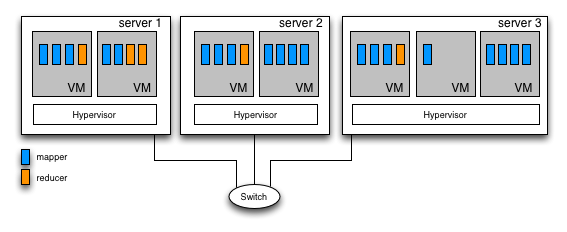
\includegraphics[width=0.5\textwidth]{figures/cluster_snapshot.png}
    \caption{\textit{An example snapshot of a running virtualised MapReduce cluster}}
    \label{cluster_snapshot}
\end{figure}

% Need a glue paragraph here

Measuring the performance of a distributed application is hard, and it is even harder when that application is running on virtualized platform which involving layers and layers of different technologies. Yet the measurement is necessary to have a proper understanding on performance of Big Data applications in the virtualized environment. Figure 1 is an abstract snapshot of a small big data application operating in virtualized environment at a random time. There are n physical servers which host multiple Virtual Machines on each of them. These VMs were set-up to run a big data application which involved many parallel tasks executing in contiguous stages. Those tasks were spawn as threads and concurrently competing for the same resources at each physical host such as disk storage, memory, and CPU,... When looking at the whole picture, we see that the performance of the whole cluster at each stage is depended on the performance of every one of its building block: one single physical host. We would like to see the different in storage I/O performance between virtualization platform and bare-metal system with the big data workloads so we designed a synthesis big data workload and run our measurements with two scenarios for virtualization and one screnario for bare-metal:
\begin{itemize}
\item Single VM with multiple threads (SVM-MT): this scenario (figure \ref{fig:svm-mt}) represents the case that the host has only one ``fat`` VM but this VM runs many parallel tasks at the same time. This SVM-MT scenario focuses on the guest OS scheduler since it has to switch between active threads. We consider 5 different flavors (sizes) of VM for this scenario to see how the VM's size affects on the performance.
\item Multiple VMs with single thread (MVM-ST): this scenario (figure \ref{fig:mvm-st}) represents the case that we have many ``slim`` VM and these VMs run only one task at a time inside its guest OS. They are colocated on the same host and they blindly competing for the same I/O resources. This scenario focuses on the hypervisor scheduler since the host has to switch between active VMs.
\item Bare-metal (BM): the bare-metal system is used as the baseline to make the comparison (figure \ref{fig:bm}). In case the big data application runs on a bare-metal environment, many parallel tasks running at the same time requesting for IO resources. In short, it is similar to the case of SVM-MT without the virtualized layer.
\end{itemize}
In this paper, we establish our focus only on the performance of shared storage I/O since it was thought to be one of the main bottle necks of big data application [5]. More specific, we are especially interesting in the performance of big data workload - mainly sequential read and sequential write in parallel issued from concurrent tasks - on the shared storage I/O. We consider I/O throughput as the metric to compare the performance between bare-metal and virtualized platform. We also keep our observation on the fairness of both platforms. The throughput metric expresses how well the system feed data to the threads while fairness keeps threads away from data starvation. Unfairness in treatment between processes creates a heterogeneous environment in which one process can becomes a straggler [\cite{matei08}] and heighten End-Job Time which in the end reduce the responsiveness of the application. We also consider CPU utilization, disk utilization, and the number of context switching in the experiments to "pinpoint" the components which affected most on the performance of shared I/O.

% This part talk about the expectation and the result of the paper, need to write it better
Before the study, our expectation was set on the conclusion of the overhead of virtualization on big data application workload. One part of our study repeats the findings of previous studies which show that, with proper tuning, virtualization can only reach maximum 80-90\% of bare metal performance due to the overhead that the added virtualization layer brought up. Previous studies reveal the performance of the system consider little about the different in level of concurrency and they also did not consider the big-data-application-like workload. Our studies reveal the big picture when there are different number of active threads concurrently competing for I/O. We consider three difference schedulers on the host: Noop, Deadline,and Scheduler and show the different behaviors of the baremetal and the virtualized platform in IO performance when using one scheduler. It is unexpected that using Deadline and Noop scheduler, Bare-metal can get less throughput than the VM that it hosts when level of concurrency is high. For CFQ scheduler, Bare-metal have good throughput and change little when there are many active threads executing but the VMs can get only 40\% of the total throughput that a Bare-metal can get. We see that both virtualized and bare-metal platform achieve high fairness index. There is no or very little different between bare-metal and virtualized platform in fairness index.

In the next sections, we introduce to our readers the methodologies in detail. We also present the findings and explanation for the result that we got. Finally, we summarize our work at the last section and suggest the future approaches to give more meaningful results to the study.

%to cite
%[1] http://www.idgenterprise.com/report/big-data-2

%%%%%%%%%%%%%%%%%%%%%%%%%%%%%%%%%%%%%%%%%%%%%%%%%%%%%%%%%%%%%%%%%%%%%
\section{Background and Related Work}
%%%%%%%%%%%%%%%%%%%%%%%%%%%%%%%%%%%%%%%%%%%%%%%%%%%%%%%%%%%%%%%%%%%%%
\begin{itemize}
  \item introduce some related works on the performance of virtualization: work from IBM on performance of KVM, work from a guy discussing the relevant of IO schedulers to virtualization system.
  \item introduce some related works on measuring performance of data intensive application
 \item then mention about the combined of both, what we are different from previous works, what are our interesting points.
\end{itemize}

In the Big Data world, data volume is too big that people avoiding moving it. With the belief that network is the bottleneck of the distributed systems, the developers try to work around by moving the execution/programs to the data but not the other way round (like Hadoop or Spark). By such method of task distributing, the burden was shifted to storage I/O (disk and memory) performance. A typical example is Hadoop with data-locality awareness. It reported achieving greater throughput when utilising data locality[?-?]. But then it makes disk I/O become the bottle-neck. Data was read from disk, intermediate data was stored on disk, and results were written to disk. Spark has done a step further, when they leverage memory to use together with the disk, Spark reported the performance improvement up to severalfold in comparing to Hadoop with data locality awareness [?]. However, memory and cache sharing was not developed well enough to also provide fault tolerant to other big data applications but Spark. Then people use data compressing techniques to trade CPU resource for storage I/O performance. But then CPU becomes the bottle-neck [?]. The simplest model is the most efficient model. That is why many data intensive applications are still greatly depended on the hard drive performance since the developers and the administrators do not want to complicate a distributed system.

A Hadoop job insludes several phases: read (1), spill (1), merge (1), transfer (2), shuffle (1), write (1). For each phase, we have more than 1 time the job read or write data.

% Summary matei08, matei-thesis
% Summary disk_schedulers_passe
% Summary works on measurement of virtualization overhead, indicate they are not focus on big data workload, most of them are white paper.

% What we different from other works? we focus on Big Data wordload, we make a simulated workload represented Hadoop and run the measurement on that workload.

% cite: Locality-Aware Reduce Task Scheduling for MapReduce - Mohammed Hammoud, CloudCom
% cite: Purlieus: Locality-aware Resource Allocation for MapReduce in a Cloud - Balaji Balanisamy
% cite: Locality-Aware Dynamic VM Reconfiguration on MapReduce Clouds - Jongse Park

%%%%%%%%%%%%%%%%%%%%%%%%%%%%%%%%%%%%%%%%%%%%%%%%%%%%%%%%%%%%%%%%%%%%%
\section{Problem statement}

A typical advice for every administrators when deploying big data application is: do not virtualize your clusters. But cloud is the trending now and avoiding virtualizing the cluster is sometimes impossible for small vendors or also for big vendors when they want to use the same infrastructure for every teams in their organization. The reason for a ``no-no`` is that big data application utilises data locality to improve performance while cloud often uses remote storages to increase high flexibility and high availability. In order to keep data locality feature, the VM instances were setup to opererate on local hard drives and it creates a situation in which many concurrently processes competing for IO resources with an intensive data volume. We designed a synthesis big data workload and do the experiments to compare between virtualized platform and bare-metal. We found that virtualization overhead is impossible to avoid. However, we can reduce the impacts by selecting the optimized I/O scheduler, the optimized flavors for the VM instances, and a good ``write-cache`` technique.

When running data intensive application in virtualized environment, the situation is worse since many VMs are sharing the same resource.
And the goal of using virtualization is to share the same resource for many users.  But we are often oversubscribing the same resource (allocate too many VM on the same physical host) to get the most out of the system performance. Given the context that many big data application are still greatly depended on disk I/O performance, we wonder how virtualization can affect on the I/O performance delicated to big data application. An experimental study of virtualization overheads for I/O operations can help to answer this question. From the characteristic of the big data application's workload, we model a simple systhesis workload that can be seen at the disk level (describe the workload here). We want to have the typical I/O ``pressure'' that comes from data-intensive applications.

Is it worthy to trade performance for virtualization benefits (resource consolidation, dynamic resource allocation, avoiding under-utilized dedicated hardware resource, improving service availability)?
% What causes overhead
``Seeing double`` problem: There may be two file systems. The guest file system and the host file system which holds the image file. There may be two volume managers. The guest and host can both use ``LVM`` and ``md`` independently. There are two page caches. Both guest and host can buffer pages from a file. There are two I/O schedulers. The guest will reorder or delay I/O but the host will too. Configuring either the guest or the host to bypass these layers typically leads to best performance.

Adding layers of complexity: 
- Extended Page Tables (EPT) add a level of address translation for guest physical memory. Guest memory address -> Guest Page Table -> Host Page Table -> Physical memory
- VM management: Switching between VMs, host hardware access and resource management  

Given the knowledge about performance bottlenecks and eventual overheads of virtualization, we can clear the myths about performance of Big Data on virtualized platform. We can also inform the users to select the best strategy for them when installed Big Data Application on the cloud respecting to optimizing the I/O performance.

%Guide from P.Pietro: Even we looking at the application level. Measure the impact of virtualization on the big data technology. we still need a proper understanding on what happens without the application because the application is very complex. it's a large distributed system that hides a lot of details so whenever you see the result, the problem is that it's very hard to explain what happened if you only look from the perspective of Hadoop or Spark. That was the reason why we simplify the thing. Let try to somehow emulate  what is the traditional workload generated by application such as Hadoop MapReduce. The question was what happens when you have the virtualization layer that hide in the middle between your application and IO call. And that why we have the measurement of bare-metal with several different configuration of the hard drive setting and CPU setting. We show that more or less the performance did not change much. So bare metal is really stable. And then we have result that look at different flavors of CPU of virtual machine with different size. And also the number of concurrent threads. These are the useful foundation for understanding the next result that you will obtain by running some sample of map reduce application which have similar workload. State what your goal are. You establish a measurement methodology where you explain your experimental setup, your tools, metrics, why they're important. And there you explain the statistical perspective of experiments. Then to validate your initial claim once the paper is done in the introduction (for example "we see that Hadoop on virtualization is suck"). You anticipate the result.

%%%%%%%%%%%%%%%%%%%%%%%%%%%%%%%%%%%%%%%%%%%%%%%%%%%%%%%%%%%%%%%%%%%%%

%%%%%%%%%%%%%%%%%%%%%%%%%%%%%%%%%%%%%%%%%%%%%%%%%%%%%%%%%%%%%%%%%%%%%
\section{The methodology}

\subsection{The system under measurement}

Our system runs on a dual hexa-core Xeon E5-2650L (with hyperthreading enabled) server clocked at 1.8GHz, with 128GB of RAM, ten 1TB disks. Disks are all the same make and model, across the hosts: SEAGATE ST91000640SS. The hardware RAID controller is configured with RAID 0 for each disk with write-back cache enabled. For easy interpreting the results, only one hard drive is use to host the VMs running the experiments. We also avoid  CPU and memory over-commit to make sure that our results were not affected by memory and CPU bottlenecks. The host machine runs the latest long term support Ubuntu 14.04 distribution, updated with the most recent patches. QEMU is used as the virtualizer to executing the guest code directly on the host CPU using the KVM kernel module in Linux. All energy saving settings in the BIOS are disabled, since they cause severe performance penalties. It uses the KVM hypervisor, with \texttt{virtio} and \texttt{vhost\_net} acceleration modules enabled. Virtualization support in the CPUs is enabled (VMX) and KVM uses it automatically. The hypervisor is configured to use LVM for VM storage. DevStack, which is an collection of scripts to quickly create an OpenStack development environment, was used to manage the deployment of VMs on the host. I/O scheduler is disable in guests' OS (in fact the guests' OS uses noop scheduler, a very simple FIFO scheduler) , and we switch between three different I/O schedulers of the host: Noop, Deadline, and Completed Fair Queueing (CFQ) to run experiments.
\subsection{Overview on the components involved}

  Application and guest kernel work similar to bare metal. Guest talks to QEMU via emulated hardware. QEMU performs I/O to an image file on behalf of the guest. Host kernel treats guest I/O like any userspace application. Therefore, the I/O performance of the guests is depended greatly on the host's I/O schedulers. Understanding how I/O schedulers works, how the kernel seeing a guest as an application, how the guest runs on the host can help to pinpoint the overheads of the virtualized platform.

  \subsubsection{Linux IO Schedulers}

    \paragraph{CFQ scheduler}
    The CFQ I/O scheduler is one of the most sophisticated I/O schedulers. The CFQ I/O scheduler divides the available I/O bandwidth among all of the processes that issue I/O requests. The CFQ I/O scheduler maintains per-process queues for synchronous I/O requests. The maximum number of per-process queues that the CFQ I/O scheduler maintains for synchronous I/O requests is 64. The CFQ I/O scheduler batches together asynchronous requests from all processes based on the priorities of the processes. For example, the CFQ I/O scheduler maintains one process queue for all asynchronous requests from processes with the idle scheduling priority.
    During each cycle, the CFQ I/O scheduler moves one request from each queue to the dispatch queue. After the CFQ I/O scheduler moves a request from each queue, it repeats the process and removes another request from each queue. After the CFQ I/O scheduler moves requests to the dispatch queue, it sorts the requests to minimize disk seeks and then services the requests accordingly. The CFQ I/O scheduler provides each queue with time to access the disk. The length of time depends on the scheduling priority of the process.
    CFQ places synchronous requests submitted by processes into a number of per-process queues and then allocates timeslices for each of the queues to access the disk. The length of the time slice and the number of requests a queue is allowed to submit depends on the I/O priority of the given process. Asynchronous requests for all processes are batched together in fewer queues, one per priority. While CFQ does not do explicit anticipatory I/O scheduling, it achieves the same effect of having good aggregate throughput for the system as a whole, by allowing a process queue to idle at the end of synchronous I/O thereby "anticipating" further close I/O from that process. It can be considered a natural extension of granting I/O time slices to a process.

    \paragraph{Deadline scheduler}
    The Deadline I/O scheduler is one of the most sophisticated I/O schedulers. The Deadline I/O scheduler dispatches I/O requests based on the length of time that the I/O requests are in the queues. Therefore, the Deadline I/O scheduler guarantees a start service time for each I/O request. The Deadline I/O scheduler maintains the deadline queues by the expiration times, or deadlines, of the I/O requests and the other queues by the positions of the requests on the disks, or sector numbers. Each set of queues, deadline queues and other queues, includes read queues and write queues. The read queues contain read requests. Because processes often block on read operations, the Deadline I/O scheduler prioritizes read requests higher than write requests and assigns read requests shorter expiration times than write requests. The write queues contain write requests.

    Based on prioritization and expiration times, the Deadline I/O scheduler determines which request from which queue to dispatch. The Deadline I/O scheduler checks to see if the first request in the deadline queue expired. If the first request in the deadline queue expired, then the Deadline I/O scheduler services the first request in the deadline queue immediately. Otherwise it services the first request from the sorted queue. To improve disk efficiency, the Deadline I/O scheduler not only services one request but also services a batch of requests near the disk location of the request that it has just taken at the top of the queue.

    \paragraph{NOOP scheduler}
    The NOOP scheduler is the simplest I/O scheduler for the Linux kernel. It inserts all incoming I/O requests into a simple FIFO queue and merges them. This scheduler is useful when it has been determined that the host should not attempt to re-order requests based on the sector numbers contained therein. In other words, the scheduler assumes that the host is unaware of how to productively re-order requests. Since I/O requests are potentially re-scheduled at the lower level, resequencing I/O request at the host level can create a situation where CPU time on the host is being spent on operations that will just be undone when they reach the lower level, increasing latency/decreasing throughput for no productive reason.

  \subsubsection{The path of a I/O request}
  
  When a VM is created, QEMU (the userspace process that performs most device emulation and controls the guest) creates a process and forks a number of vCPU threads associating with same number of virtual cpu that the VM was allocated. These dedicated vcpu threads use the kvm.ko module in the kernal to execute guest code. Besides, the ``iothread`` thread is created for handling IO for this virtual machine. There is an I/O thread that runs a select loop to handle events. Only one thread may be executing QEMU code at any given time. This excludes guest code and blocking in select.

  Application and guest kernel work similar to bare metal. Guest talks to QEMU via emulated hardware. QEMU performs I/O to an image file on behalf of the guest. Host kernel treats guest I/O like any user space application. QEMU presents emulated storage interfaces to the guest. Virtio is a paravirtualized storage interface, delivers the best performance. One virtio-blk PCI adapter per block device

  % Rewrite everything for this. Clarify how a request was submitted to the host. Then look for information how IO request was handle at the host. Remember to insert picture for easier understanding.

\subsection{The measurement methodology}

\subsubsection{Tools}

We relies on FIO for disk measurement in this paper. FIO is short for Flexible I/O, a versatile I/O workload generator. It was written to benchmark or verify changes to the Linux IO subsystem by Linux developers. FIO is flexible enough to allow detailed workload setups, and it contains the necessary reporting to make sense of the data at completion. FIO is widely used as an industry standard benchmark, stress testing tool, and for I/O verification purposes. FIO isn't tied to any OS. It works on any platform from Windows to HP-UX to Android. There are also native IO engines on Linux, Windows, Solaris, etc. This is a key feature to allow many kinds of measurement repeatable across platforms. Besides, FIO supports three different types of output format: the default console output which dumps workload statistics at the end of the run, the file output with CSV format called Terse, and the JSON-based output file format which is far more flexible and has the advantage of being simple to parse for people and computers. However, JSON format only available in later version of FIO. We prefer the Terse format since it is available to more versions of FIO which can help us easily migrate our micro benchmark script to different platforms.

\subsubsection{Scenarios and Experiment Design}

We run FIO on the physical host with different number of FIO threads (from 1 to 16 concurrent threads). Then with the same configuration, we run it on 5 different VM flavors (VM with one, two, four, eight, and sixteen cores). We also make the comparison with the case that each VM has only one thread but we use many concurrent active VMs on the same host to perform I/O operation. We use identical Operating Systems and identical OS' setting across platforms to make sure that the measurement result is reliable. The same fixed amount of data was used throughout the test. When there are many concurrent threads or concurrent VMs running in one test, we distribute the input data equally to all of them.

With the described scenarios above, we group our tests into three scenarios:
\begin{itemize}
  \item \textbf{Bare-metal (BM)}: multiple threads concurrently read data from or write data to the disk. Data were read from or written to a directory placed on the same hard drive.

  \item \textbf{Single VM with multiple threads (SVM-MT)}: 5 different default VM flavors of OpenStack (each flavor has different number of core) ran the same test with the involvement of 1 to 16 threads. Details on the specs of the flavors can be seen on table [?]. The first line is the name of the flavors.
      \begin{table}[h!]
      \begin{tabular}{|l|c|c|c|c|c|}
      \hline
      Resource & small & medium & large & xlarge & xxlarge \\
      \hline
      vCPU & 1 & 2 & 4 & 8 & 16 \\
      Memory (GB)& 1 & 4 & 8 & 16 & 16 \\
      Disk (GB)& 40 & 40 & 40 & 40 & 40 \\
      \hline
      \end{tabular}
      \end{table}
  \item \textbf{Multiple VMs with a single threads (MVM-ST)}: 16 low-specs VMs, each VM initiates only one process to read/write data. We would like to prevent the CPU becoming the bottle neck so we use the ``small`` flavor in this screnario with only one vCPU and 1GBs of memory.
\end{itemize}

\begin{figure*}[t]
   \centering
   \begin{subfigure}[b]{0.3\textwidth}
     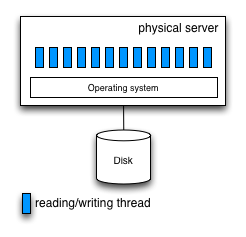
\includegraphics[width=\textwidth]{figures/bare-metal.png}
     \caption{\textit{Bare-metal scenario}}
     \label{fig:bm}
   \end{subfigure}%
   ~ %add desired spacing between images, e. g. ~, \quad, \qquad, \hfill etc.
     %(or a blank line to force the subfigure onto a new line)
   \begin{subfigure}[b]{0.3\textwidth}
     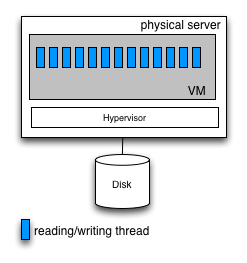
\includegraphics[width=\textwidth]{figures/SVM-MT.png}
     \caption{\textit{SVM-MT scenario}}
     \label{fig:svm-mt}
   \end{subfigure}
    ~ %add desired spacing between images, e. g. ~, \quad, \qquad, \hfill etc.
      %(or a blank line to force the subfigure onto a new line)
   \begin{subfigure}[b]{0.3\textwidth}
     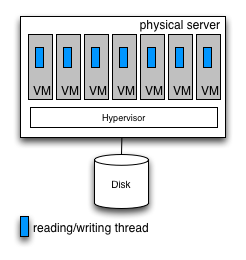
\includegraphics[width=\textwidth]{figures/MVM-ST.png}
     \caption{\textit{MVM-ST scenario}}
     \label{fig:mvm-st}
   \end{subfigure}
   \caption{Three scenario in the measurement}\label{fig:scenario}
\end{figure*}

FIO runs a job after reading the setting for the jobs from a configuration file. Our sample configuration file was follow this sample:
\begin{lstlisting}
  ; sample setting of one thread
  [sequential-read] ; name of the thread
  rw=read             ; use sequential read
  size=(4Bb/num_threads) ; size read/written per thread
  directory=/fiotest; directory for read/write
  ioengine=libaio     ; I/O engine
  direct=1            ; disable OS buffering
  iodepth=32          ; in-flight IO requests per threads
\end{lstlisting}

Where:
\begin{itemize}
  \item \textbf{rw} defines the kind of disk access pattern: read (sequential reads), write (sequential writes), randread (random reads), randwrite (random writes), or mixed. We specially focus only on the two basic access patterns which happen mostly in the context of Big Data world: sequential read and sequential write. A typical example is the Hadoop File System (HDFS) which writes data in large contiguous chunks on disk, which in turn means data is written and read in large sequential operations. For HDFS, this minimizes drive seek operations — one of the slowest operations a mechanical disk can perform — and results in better performance when streaming data to workers (locally or remotely) \ref{chapter2-HDFS-HadoopOperationBook}.
 \item \textbf{size} is the total size of input data for this job. FIO will run until this many bytes of data has been transferred. We choose the total transfer volume to be 4 GBs. This is large enough to avoid many kinds of buffering from the application layer to the OS layer and then to the hardware layer. The total amount of data will be distributed equally to all the parallel threads that join the test.
  \item \textbf{direct I/O} set the value of O\_DIRECT in the Linux kernel. I/O operations performed against files opened with O\_DIRECT bypass the kernel's page cache, writing directly to the storage. Recall that the storage may itself store the data in a write-back cache (in our case, the storage has 64 MBs of write-back cache). There is no strict guarantee that the function will return only after all data has been transferred.
  \item \textbf{iodepth} defines the I/O depth of the system. This defines how many IO requests to keep in flight against the file. The default is 1 for each file defined in the job description. This value can be overridden with a larger value for higher concurrency. We use I/O depth of 32 after run some initial tests to get the setting of the maximum performance of the disk. In fact, the default I/O depth in some of the Linux distributions can even be set upto 256 or 512.
  \item \textbf{ioengine} is \texttt{libaio} which indicates the application to use AIO (Asynchronous Linux I/O) subsystem. AIO helps to overlaps processing with I/O Operations. Application can submit (batch of) I/O operation without waiting for completion. This benefits physical I/O in particular when prefetching data. Besides, it allows to accumulate read or write requests so that the I/O subsystem can optimize performance by grouping or reordering the IO requests in favor of sequential access and large request. It helps to separate calls for submission and completion indication and pipelines operations to improve throughput. It also helps to improved utilization of CPU and devices.
\end{itemize}

\subsection{The performance/overheads metrics}

During these measurements all VMs were using logical volumes created on the same physical hard disk. Physical CPU cores are not reserved for each VM, but during measurements there was enough spare capacity available to guarantee that each VM had enough cores (as configured by the VM flavor) available for its exclusive use.

\paragraph{Aggregated Throughput}
We considered the aggregated throughput is a good metrics to compare the scenarios. We run our measurement 10 times, for each run we collect the aggregated throughput of all threads and calculate the aggregated throughput. All of our figures was plotted with 95\% of confident interval.

\paragraph{Jain Fairness Index}
  To evaluate fairness, we rely on the Jain Fairness Index \ref{jain}, which is defined as
  $$JFI={({\sum}_{i}x_{i})^{2}\over n{\sum}_{i}x_{i}^{2}}$$
  where $x_{i}$ is the average throughput of the $i^th$ flow and $n$ the number of parallel threads. It features interesting properties when one wants to assess the fairness of a system. If all samples (throughput values in our case) are equal, the Jain Fairness index is simply 1, which is its maximal possible value. Also, the minimal value of the JFI is $\frac{1}{n}$. JFI is very important because its can cause stragglers in big data application. Straggler is created when a task does not receive the same amount of data as other tasks, it cannot perform its task and let the whole execution process to wait for its result. This increase the completion time of the whole job.
%%%%%%%%%%%%%%%%%%%%%%%%%%%%%%%%%%%%%%%%%%%%%%%%%%%%%%%%%%%%%%%%%%%%%

%%%%%%%%%%%%%%%%%%%%%%%%%%%%%%%%%%%%%%%%%%%%%%%%%%%%%%%%%%%%%%%%%%%%%
\section{Results}

\subsection{Aggregated Throughput}

\begin{figure*}[t]
   \centering
   \begin{subfigure}[b]{0.3\textwidth}
     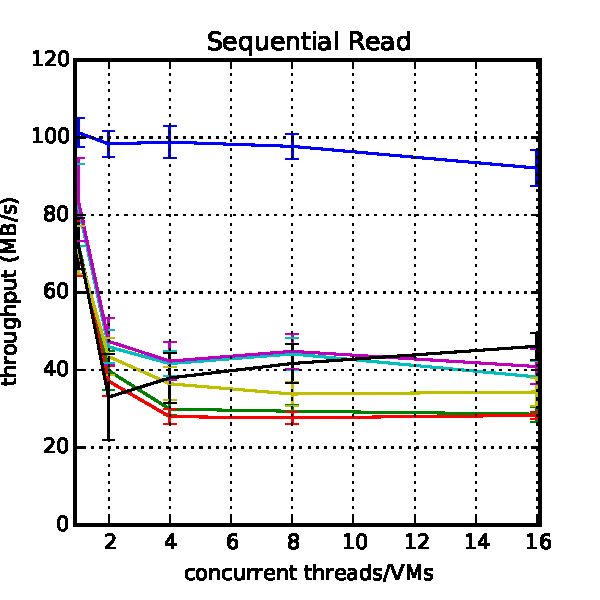
\includegraphics[width=\textwidth]{figures/throughput_cfq_read.pdf}
     \caption{CFQ}
     \label{fig:aggthroughput_cfq_read}
   \end{subfigure}%
   ~ %add desired spacing between images, e. g. ~, \quad, \qquad, \hfill etc.
     %(or a blank line to force the subfigure onto a new line)
   \begin{subfigure}[b]{0.3\textwidth}
     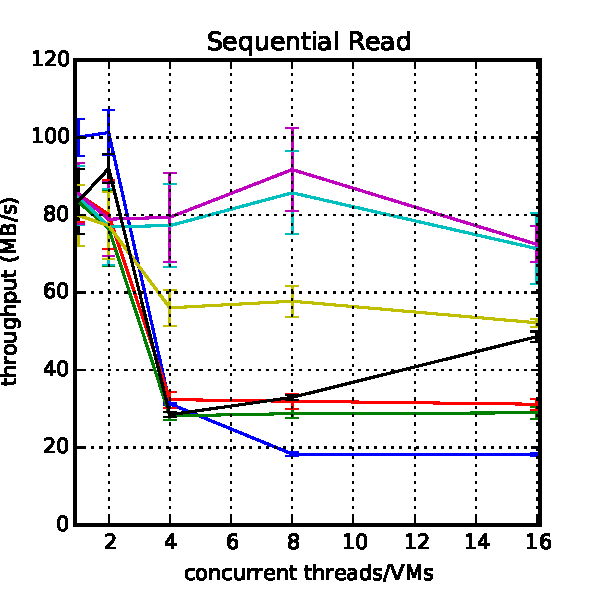
\includegraphics[width=\textwidth]{figures/throughput_deadline_read.pdf}
     \caption{Deadline}
     \label{fig:aggthroughput_dealine_read}
   \end{subfigure}
    ~ %add desired spacing between images, e. g. ~, \quad, \qquad, \hfill etc.
      %(or a blank line to force the subfigure onto a new line)
   \begin{subfigure}[b]{0.3\textwidth}
     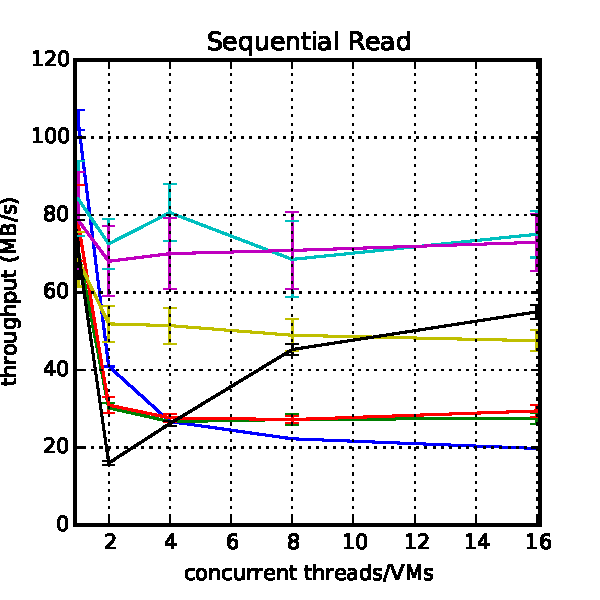
\includegraphics[width=\textwidth]{figures/throughput_noop_read.pdf}
     \caption{Noop}
     \label{fig:aggthroughput_noop_read}
   \end{subfigure}
   \hfill
   \begin{subfigure}[b]{0.3\textwidth}
     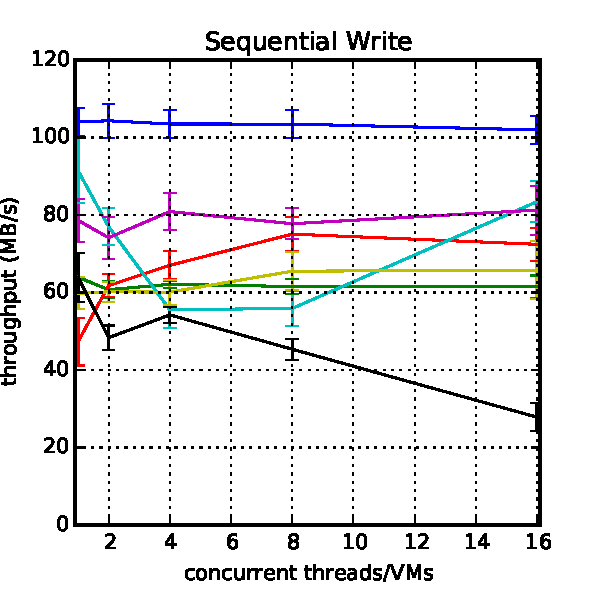
\includegraphics[width=\textwidth]{figures/throughput_cfq_write.pdf}
     \caption{CFQ}
     \label{fig:aggthroughput_cfq_write}
   \end{subfigure}%
   ~ %add desired spacing between images, e. g. ~, \quad, \qquad, \hfill etc.
     %(or a blank line to force the subfigure onto a new line)
   \begin{subfigure}[b]{0.3\textwidth}
     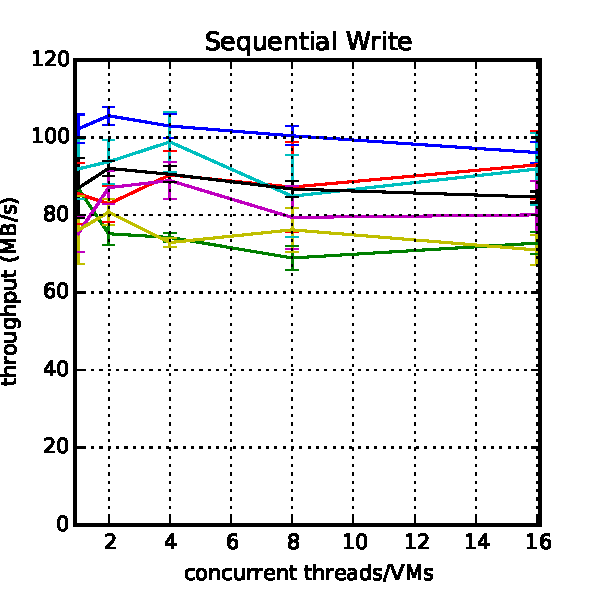
\includegraphics[width=\textwidth]{figures/throughput_deadline_write.pdf}
     \caption{Deadline}
     \label{fig:aggthroughput_deadline_write}
   \end{subfigure}
    ~ %add desired spacing between images, e. g. ~, \quad, \qquad, \hfill etc.
      %(or a blank line to force the subfigure onto a new line)
   \begin{subfigure}[b]{0.3\textwidth}
     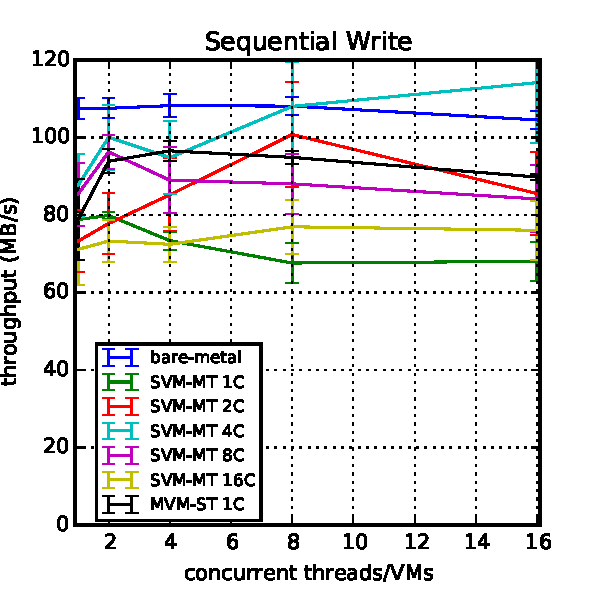
\includegraphics[width=\textwidth]{figures/throughput_noop_write.pdf}
     \caption{Noop}
     \label{fig:aggthroughput_noop_write}
   \end{subfigure}
   \caption{Aggregated throughput with the three I/O schedulers}\label{fig:aggthroughput}
\end{figure*}

\paragraph{Sequential Read}
We presented in figure \ref{fig:aggthroughput} the average aggregated throughput of our systems with three I/O schedulers on the host: CFQ, Noop, and Deadline respectively. For the 3 figures, we see two different behaviors of the virtualized platforms and the baremetal one. On one hand, the baremetal have very good performance with the CFQ scheduler, but it is not the same for the performance of the virtualized one. In all of the screnarios, the virtualized platform only gets about 40\% of aggregated throughput when number of parallel thread is increased. On the other hand, bare-metal system does not perform well with the Noop and Deadline scheduler. It is downgraded to 35\% at 4 parallel threads and to 19\% at more than 8 parallel threads. The virtualized platform sees a discrepancy at 4 parallels threads between different flavors. Flavors with 4 and 8 virtual cores can keep the aggregated throughput stable at 80MB/s with the increment of concurrency level. Flavors with 1 and 2 cores get low performance at 28MB/s, but still higher than the bare-metal one. The flavor of 16 cores was expected to have the greatest throughput, but it does not. Its performance is in the middle of the one with 4 or 8 cores and the one with 1 or 2 core. The case of MVM-ST is very weird when it gets low throughput at 17MB/s with 2 parallel threads but recover after the number of parallel threads increases.

\paragraph{Sequential Write}
For sequential write, the performance of bare-metal does not change between the host schedulers. Yet the performance of virtualized platform is a little better around 85 MB/s for Deadline and Noop in compare with the aggregated throughput at around 70 MB/s when with CFQ scheduler.
For this access pattern, we see that the performance is affected mostly by write-back cache and write-through cache of the the RAID controller device. Noted that there are three main caching techniques that can be deployed nowadays as mentioned in details below:
\begin{itemize}
  \item \textbf{Write-through cache} directs write I/O onto cache and through to underlying permanent storage before confirming I/O completion to the host. This ensures data updates are safely stored on the storage device, but has the disadvantage that I/O still experiences latency based on writing to that storage.
  \item \textbf{Write-around cache} is a similar technique to write-through cache, but write I/O is written directly to permanent storage, bypassing the cache. This can reduce the cache being flooded with write I/O that will not subsequently be re-read, but has the disadvantage is that a read request for recently written data will create a ``cache miss`` and have to be read from slower bulk storage and experience higher latency.
  \item \textbf{Write-back cache} is where write I/O is directed to cache and completion is immediately confirmed to the host. This results in low latency and high throughput for write-intensive applications, but there is data availability exposure risk because the only copy of the written data is in cache. Write-back cache is the best performing solution for mixed workloads as both read and write I/O have similar response time levels.
\end{itemize}

We presented the IO performance of sequential write when we using write-through cache in figure \ref{fig:throughputwritethrough}.

\begin{figure}[htbp]
  \centering
  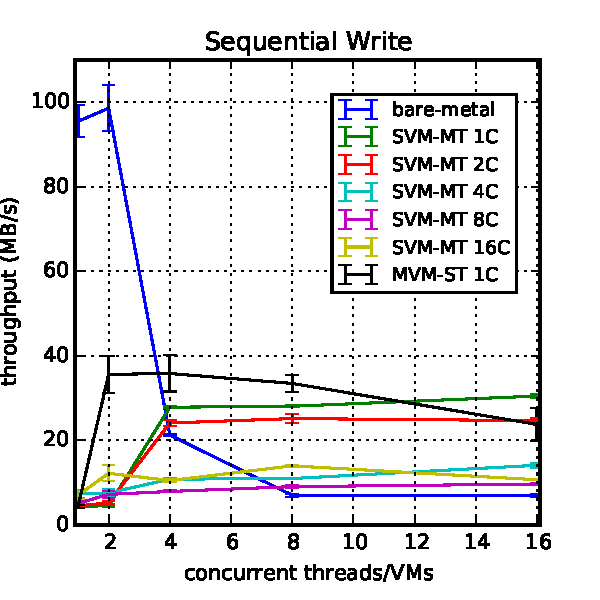
\includegraphics[scale=0.7]{figures/throughputwritethrough.pdf}
  \caption{\textit{Write-through cache is using on the host and the VMs}}
  \label{fig:throughputwritethrough}
\end{figure}

\paragraph{Discussion}
To explain for the result that we got, we have ask ourselves many questions:
\begin{itemize}
 \item \textit{In case of using Deadline and Noop scheduler, why there is different behavior for different VM flavors of SVM-MT scenario?}
 \item \textit{We see that IO performance is changed when VMs have different number of cores. Do reducing the number of online (not-disable) cores on bare-metal will reduces IO performance of bare-metal?} we reduced the number of online cores on bare-metal to see if IO performance of bare-metal is affected. However, for all the different numbers of online cores on the bare-metal, we still get similar throughput. (Figure \ref{fig:throughputbmdiffonlinecore})
     \begin{figure*}[t]
      \centering
      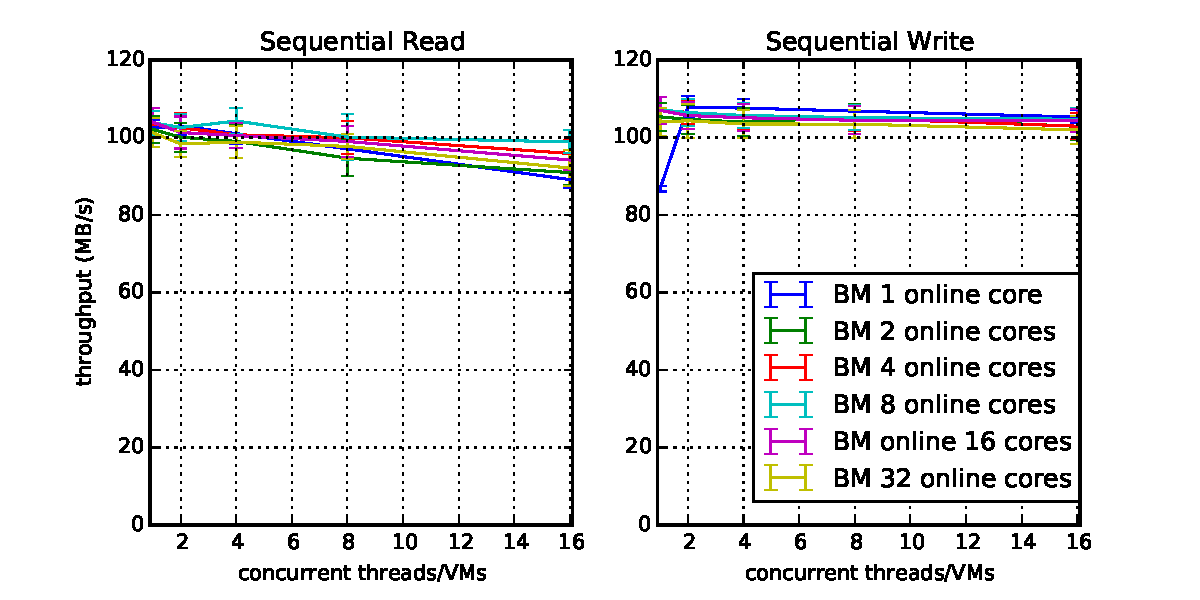
\includegraphics[scale=0.7]{figures/throughput_cfq_bmdiffonlinecore.pdf}
      \caption{\textit{Throughput of baremetal with different number of online cores}}
      \label{fig:throughputbmdiffonlinecore}
     \end{figure*}
 \item \textit{Why does the deadline scheduler and Noop scheduler has similar result?} The Deadline elevator uses a deadline algorithm to minimize I/O latency for I/O requests. A standard elevator algorithm is used, unless the request at the head of one of the FIFO queues grows older than an expiration value. In that case the scheduler begins servicing expired requests. The results shown in this study show the Deadline scheduler behaving almost identically to the Noop scheduler. It seems likely that the deadlines imposed by the scheduler are never exceeded, resulting in the Deadline scheduler devolving to the same behavior as the Noop scheduler.
 \item \textit{Why does throughput reduce after 2 concurrent threads?} % We should trade the instruction latencies. This is very similar to a white paper of Ebay Inc.
 \item \textit{What exactly is happening at the hypervisor level in the scenario with MVM-ST? Why do we have an increasing trend?}
 \item \textit{Why is READ performance worse than WRITE?} For write performance, we are writing to the cache of the RAID controller, but not actually writing to the disk. It is clearly showed in the figure with the cache-through technique (figure \ref{fig:throughputwritethrough}), when the OS waits for system calls return after the I/O request was written successfully to disk, we have less output.
 \item \textit{Is the disk or the vdisk the bottleneck?} % To answer this, we need to find the disk utilization from the perspectives of both the guest OS and host OS.
 \item \textit{Is the CPU or vCPU the bottleneck?} % To answer this, we need to find the CPU utilization from the perspectives of both the guest OS and host OS.
 \item \textit{Why does SMV-MT scenario got low throughput when using CFQ scheduler at the host?} CFQ scheduler maintains 64 per-process queues for synchronous IO request while it only maintains one queue for asynchronous IO request. We checked the fairness of two platforms when using CFQ and saw that BareMetal linearly reduced its fairness from 1 (at 1 thread) to 0.85 (at 16 threads) while the virtualized platform maintains its perfect fairness at 1 during the experiments (as in figure \ref{fig:jfi}). We guess that eventhough we setup FIO to use asynchronous I/O in the guest OS, but after the IO requests left the guest OS, it was treated as synchronous IO at the host domain. CFQ get perfect fairness because it serves each IO queue of each process with an equal quantum time, when using only one queue for all the processes, the system would lose its fairness. Synchronous IO has lower performance since it is a blocking mechanism.
\end{itemize}


\paragraph{CPU utilization}

For CPU utilization, FIO relies on getrusage(). Getrusage() returns resource usage statistics for the calling thread. The resource usages are returned in the structure pointed by the usage caller, which has the following form:

\begin{lstlisting}
struct rusage {
    struct timeval ru_utime; // user CPU time used
    struct timeval ru_stime; // system CPU time used
    ...
    long   ru_minflt;  // page reclaims (soft page faults)
    long   ru_majflt;  // page faults (hard page faults)
    long   ru_nswap;   // swaps
    ...
    long   ru_nvcsw;   // voluntary context switches
    long   ru_nivcsw;  // involuntary context switches
};
\end{lstlisting}

and contained inside the struct are:

\begin{itemize}
  \item \textit{ru\_utime}: This is the total amount of time spent executing in user mode, expressed in a timeval structure (seconds plus microseconds).
  \item \textit{ru\_stime}: This is the total amount of time spent executing in kernel mode, expressed in a timeval structure (seconds plus microseconds).
  \item \textit{ru\_nvcsw}: The number of times a context switch resulted due to a process voluntarily giving up the processor before its time slice was completed (usually to await availability of a resource).
  \item \textit{ru\_nivcsw}: The number of times a context switch resulted due to a higher priority process becoming runnable or because the current process exceeded its time slice.
  \item \textit{run\_time}: The duration from the time that thread starts until the time that thread finishes or the wall lock time.
\end{itemize}

FIO reports the CPU utilization for each thread by $\frac{ru\_utime}{run\_time}$ and $\frac{ru\_stime}{run\_time}$. However, we are more interested in the serving time (the time that thread actually uses the CPU) and the waiting time (the time that thread has to wait for the others until its slice is up).
\begin{lstlisting}
    serving_time = ru_utime + ru_stime
    waiting_time = run_time - serving_time
\end{lstlisting}

\paragraph{Context switching between scenarios}
Bla bla bla
\begin{figure*}[t]
   \centering
   \begin{subfigure}[b]{0.3\textwidth}
     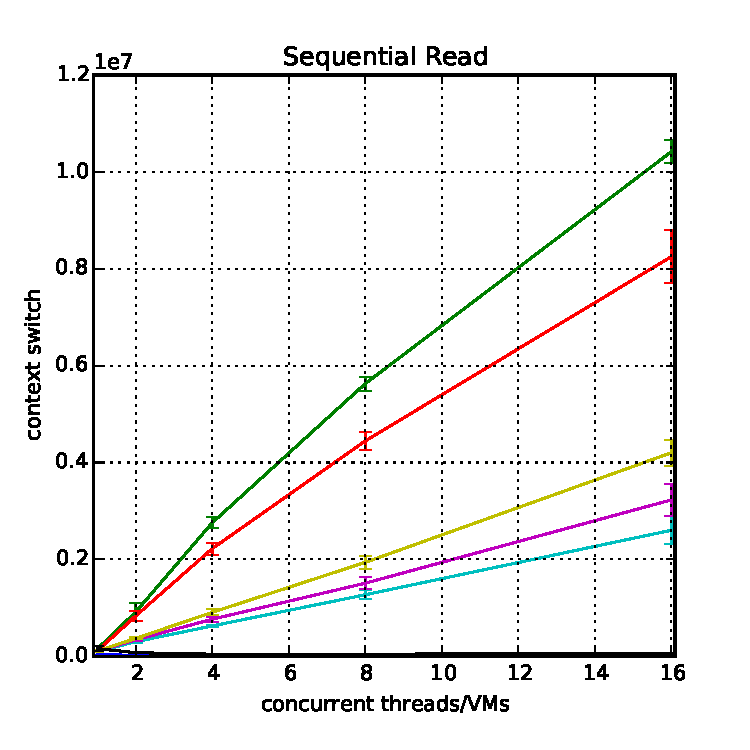
\includegraphics[width=\textwidth]{figures/contextswitching_cfq_read.pdf}
     \caption{CFQ}
     \label{fig:contextswitching_cfq_read}
   \end{subfigure}%
   ~ %add desired spacing between images, e. g. ~, \quad, \qquad, \hfill etc.
     %(or a blank line to force the subfigure onto a new line)
   \begin{subfigure}[b]{0.3\textwidth}
     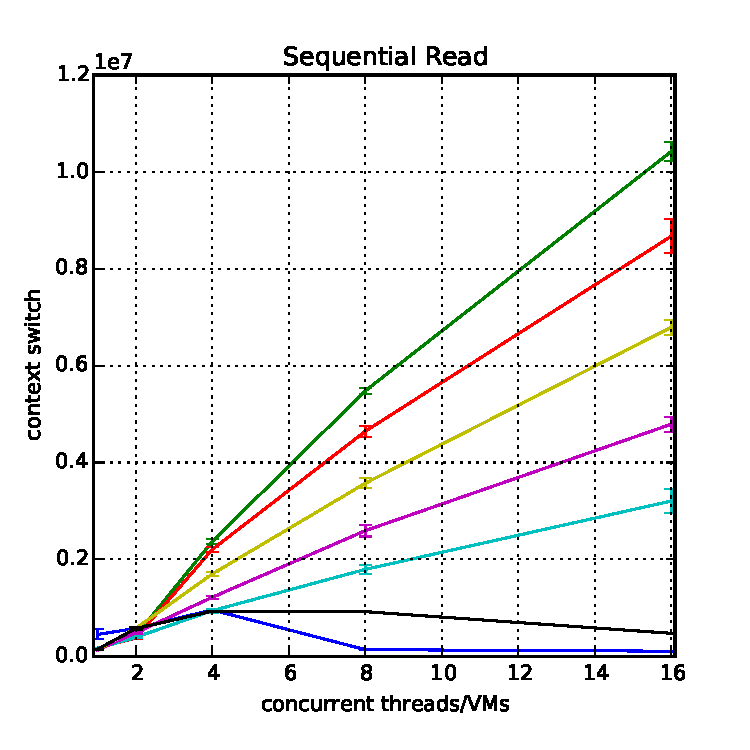
\includegraphics[width=\textwidth]{figures/contextswitching_deadline_read.pdf}
     \caption{Deadline}
     \label{fig:contextswitching_dealine_read}
   \end{subfigure}
    ~ %add desired spacing between images, e. g. ~, \quad, \qquad, \hfill etc.
      %(or a blank line to force the subfigure onto a new line)
   \begin{subfigure}[b]{0.3\textwidth}
     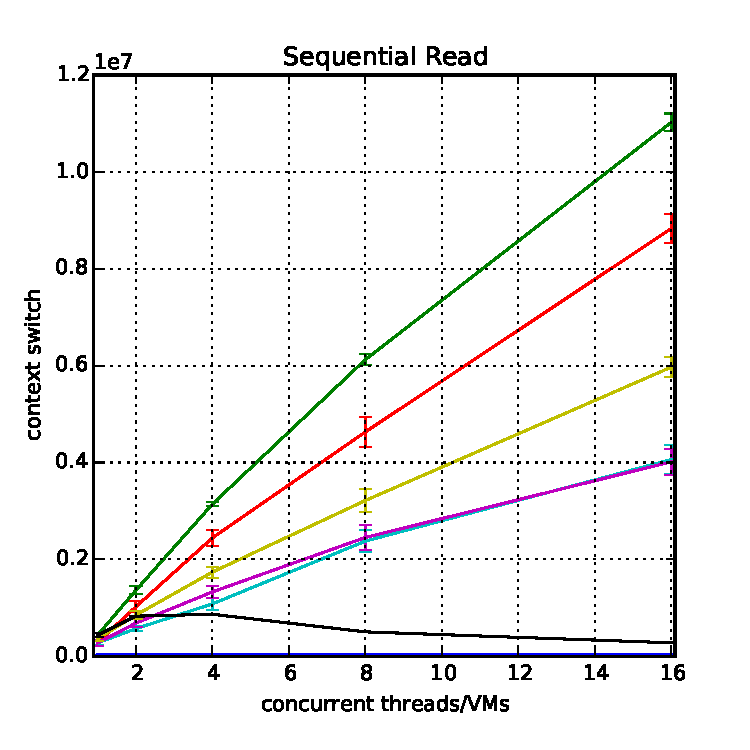
\includegraphics[width=\textwidth]{figures/contextswitching_noop_read.pdf}
     \caption{Noop}
     \label{fig:contextswitching_noop_read}
   \end{subfigure}
   \hfill
   \begin{subfigure}[b]{0.3\textwidth}
     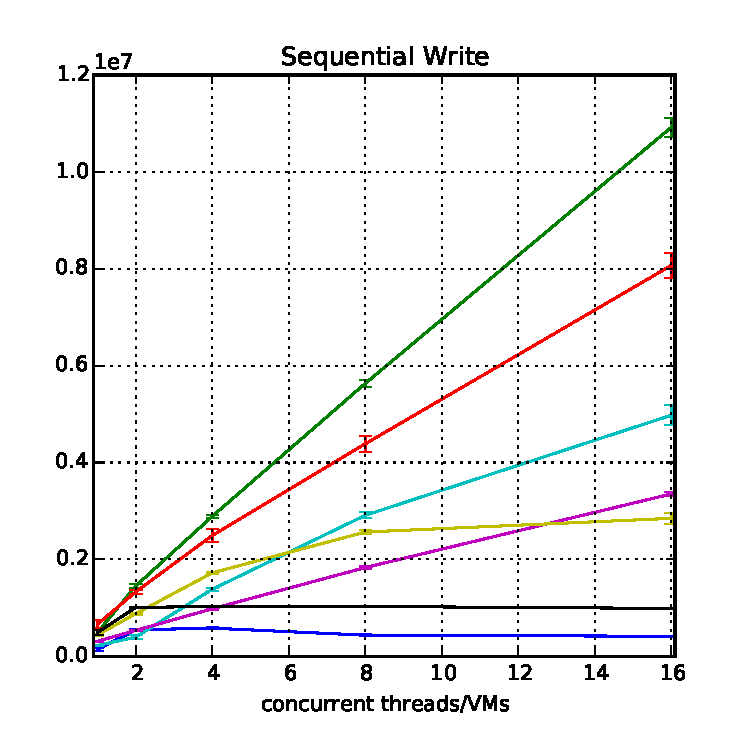
\includegraphics[width=\textwidth]{figures/contextswitching_cfq_write.pdf}
     \caption{CFQ}
     \label{fig:contextswitching_cfq_write}
   \end{subfigure}%
   ~ %add desired spacing between images, e. g. ~, \quad, \qquad, \hfill etc.
     %(or a blank line to force the subfigure onto a new line)
   \begin{subfigure}[b]{0.3\textwidth}
     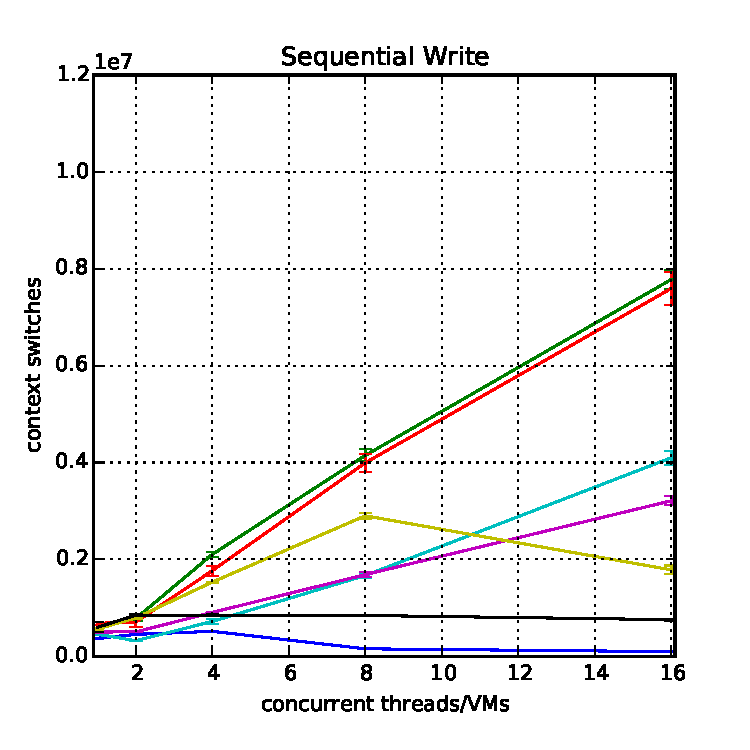
\includegraphics[width=\textwidth]{figures/contextswitching_deadline_write.pdf}
     \caption{Deadline}
     \label{fig:contextswitching_deadline_write}
   \end{subfigure}
    ~ %add desired spacing between images, e. g. ~, \quad, \qquad, \hfill etc.
      %(or a blank line to force the subfigure onto a new line)
   \begin{subfigure}[b]{0.3\textwidth}
     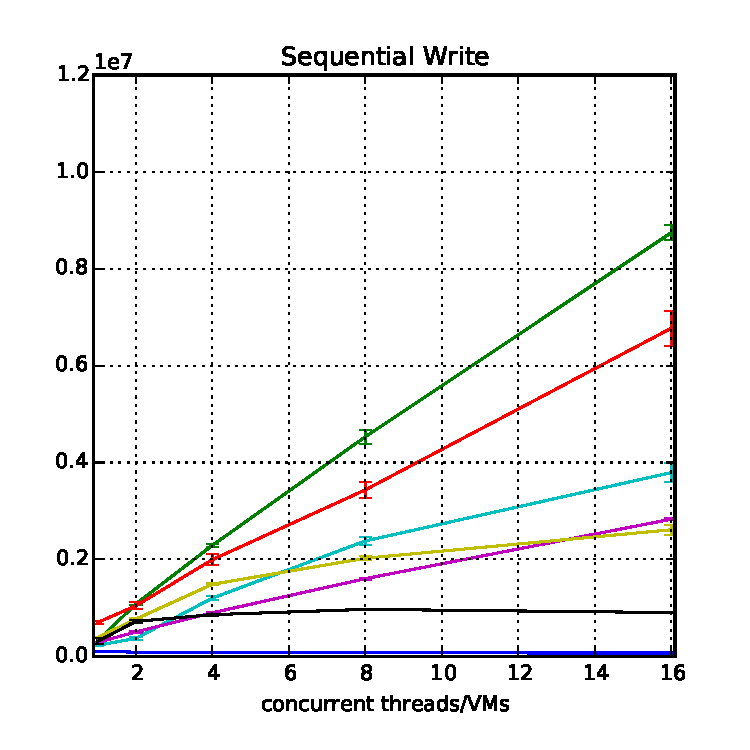
\includegraphics[width=\textwidth]{figures/contextswitching_noop_write.pdf}
     \caption{Noop}
     \label{fig:contextswitching_noop_write}
   \end{subfigure}
   \caption{Number of context switchings with the three I/O schedulers}\label{fig:contextswitching}
\end{figure*}

\subsection{Jain Fairness Index}
In our experiments, for all the I/O schedulers and platforms. Fairness index is very high. Fairness may not show much the different between bare-metal and virtualization in term of performance, but why did we select it as a metric for the comparison? Because fairness has big impacts on Big Data application. Whenever a task is not received the same amount of data as other tasks, it will become a straggler \ref{matei08}. In the context of big data application, a straggler is very bad. 1) For Hadoop and Spark, in particular, the slowest task determines the overall job completion time. Straggler causes the whole execution to wait for some slow tasks before it can finish and return the results. 2) Many systems like Hadoop and Spark deploy task speculation. This is an optimization technique to performs some tasks that may not be actually needed. The main idea is to run a task before it is known whether the results of that task will be needed, so as to prevent a delay incurred by re-run that task after it is known whether it is needed. If it turns out the work was not needed after all, any result produced by the speculative tasks is ignored. If we have a fair system, we can avoid wasting resources for the speculative tasks.
 
\begin{figure*}[t]
  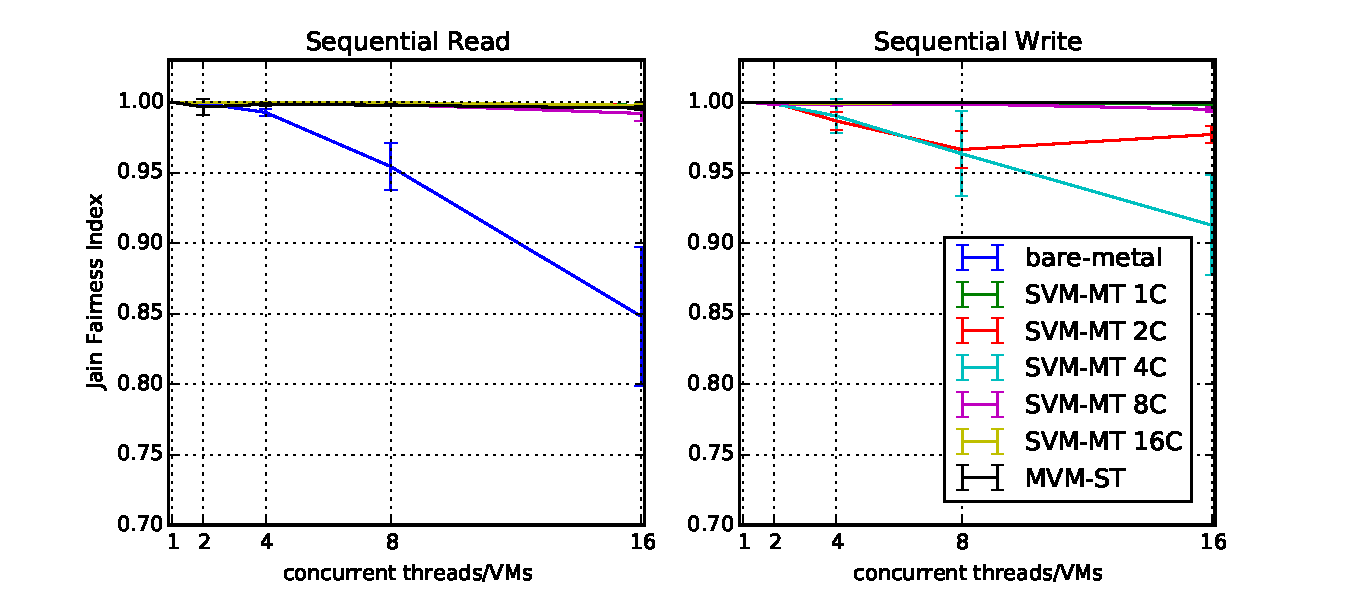
\includegraphics[scale=0.85]{figures/JFI.pdf}
  \caption{\textit{Jain Fairness Index of different scenarios with CFQ scheduler}}
  \label{fig:jfi}
\end{figure*}


%%%%%%%%%%%%%%%%%%%%%%%%%%%%%%%%%%%%%%%%%%%%%%%%%%%%%%%%%%%%%%%%%%%%%





%%%%%%%%%%%%%%%%%%%%%%%%%%%%%%%%%%%%%%%%%%%%%%%%%%%%%%%%%%%%%%%%%%%%%
\section{Conclusion}
By using a synthesis workload mimic from a MapReduce-like application, we reveal the overhead of virtualization in term of IO performance. We confirm the results of \ref{kvmperformance2013,ioschedulerpasse2010} and giving further details on the I/O performance of the virtualized and baremetal systems respected to level of concurrency and Big-data-like workload. We have found and confirmed that:
\begin{itemize}
  \item The schedulers of the host play an important role in the behavior of the performance of the system. A cloud administrator should choose Deadline of Noop scheduler for there Big Data application. If they want to use the baremetal one, CFQ is a better choice since it works well with data intensive workload. The virtualization platform achieve better aggregated throughput with Deadline and Noop scheduler. In addition, It's depended on the number of cores to achieve the greatest throughput for one VM instance in the cloud. Currently we do not have a method to select the best specs for the VM with a given host specs in favor of I/O performance. But the reader can repeat our experiment with our automated scripts \ref{link:github} to select the best flavor for their hosts.
  \item Both platform achieve great fairness index in term of IO performance. Keeping our eyes on the fairness index enables us to explain the bad performance of SVM-MT with the CFQ scheduler.
  \item For sequential write workload, we showed that the virtualized platform lose 15-30\% in compare with the bare-metal. Both platform are affected greatly by the caching technique that deploy on the RAID controller. In details, Write-back and Write-through cache play important role in the performance of sequential writing for both the bare-metal and the virtualized platform. For Hadoop-like workload, user should use write-back cache since it's perform well with data intensive workload.
\end{itemize}

We believe that the result from this work can help the communities to have deeper understanding on the performance of virtualization when they need to deploy Big Data application on the cloud. However, this is just the first part in a continuation research which studies on the impacts of virtualization on Data Intensive Analysis Framework in which there are two most popular representatives: Hadoop and Spark. Those application performance can be bounded by network, disk I/O, or CPU performance. In this paper, we focus on and only on disk I/O and it is the limitation of our work. This work is still limited in explaining the insides that cause the seperated performance between VM flavors. We also avoid memory and CPU over-commit which is happen often happen when using virtualization technology. Performance of Big Data application is not only depended on storage I/O performance, but if one component is better, the whole process should be better. In future, we would like to see how the I/O performance was seen from the perspective of the big data application (such as Hadoop or Spark). From then we can prove the correctness of our synthesis workload design.

%%%%%%%%%%%%%%%%%%%%%%%%%%%%%%%%%%%%%%%%%%%%%%%%%%%%%%%%%%%%%%%%%%%%%



%%%%%%%%%%%%
% THIS PART IS FOR THE REFERENCE SECTION
%%%%%%%%%%%%
% \balance
% \bibliographystyle{abbrv}
% \bibliography{ref}

\end{document}
